\documentclass[serif, xcolor=dvipsnames]{beamer}

\makeatletter

\documentclass[xcolor={usenames,svgnames,dvipsnames}]{beamer}
\usepackage[utf8]{inputenc}
\usepackage[T1]{fontenc}
\usepackage{graphicx}
\usepackage{grffile}
\usepackage{longtable}
\usepackage{wrapfig}
\usepackage{rotating}
\usepackage[normalem]{ulem}
\usepackage{amsmath}
\usepackage{textcomp}
\usepackage{amssymb}
\usepackage{capt-of}
\usepackage{hyperref}
\usepackage{color}
\usepackage{listings}
\usepackage{mathpazo}
\usepackage{gensymb}
\usepackage{amsmath}
\usepackage{chemarr}%flechas para reacciones químicas (SFER.tex)
\bibliographystyle{plain}
\AtBeginSubsection[]{\begin{frame}[plain]\tableofcontents[currentsubsection,sectionstyle=show/shaded,subsectionstyle=show/shaded/hide]\end{frame}}
\AtBeginSection[]{\begin{frame}[plain]\tableofcontents[currentsection,hideallsubsections]\end{frame}}
\usepackage[emulate=units]{siunitx}
\sisetup{fraction=nice, decimalsymbol=comma, retain-unity-mantissa = false}
\newunit{\wattpeak}{Wp}
\newunit{\watthour}{Wh}
\newunit{\amperehour}{Ah}
\usepackage{steinmetz}
\hypersetup{colorlinks=true, linkcolor=OliveGreen, urlcolor=Blue}
\renewcommand{\thefootnote}{\fnsymbol{footnote}}
\beamertemplatenavigationsymbolsempty
\setbeamertemplate{footline}[frame number]

\setbeamercolor{alerted text}{fg=Green!50!black} \setbeamerfont{alerted text}{series=\bfseries}
\usefonttheme{serif}
\setbeamercovered{transparent}
\setbeamertemplate{navigation symbols}{}
\usefonttheme{serif} 

\setbeamercolor{palette primary}{bg=OliveGreen,fg=white}
\setbeamercolor{palette secondary}{bg=OliveGreen,fg=white}
\setbeamercolor{palette tertiary}{bg=OliveGreen,fg=white}
\setbeamercolor{palette quaternary}{bg=OliveGreen,fg=white}
\setbeamercolor{structure}{fg=OliveGreen} % itemize, enumerate, etc
\setbeamercolor{section in toc}{fg=OliveGreen} % TOC sections

\usetheme[hideothersubsections]{Goettingen}

\usepackage{tikz}

\titlegraphic{
\includegraphics[width=2.5cm]{../figs/logoEOI.jpg}}
\addtobeamertemplate{frametitle}{}{%
\begin{tikzpicture}[remember picture,overlay]
\node[anchor=south east,yshift=2pt] at (current page.south east) {
\includegraphics[width=1.5cm]{../figs/logoEOI.jpg}};
\end{tikzpicture}}


\makeatother


\usepackage[spanish]{babel}
\addto\shorthandsspanish{\spanishdeactivate{~<>}}

\begin{document}

\title[\textsc{ESF: Componentes SFA}]{\textsc{Energía Solar Fotovoltaica:}\\
\textsc{Componentes de un Sistema Autónomo}}


\author{\textsc{Oscar Perpiñán Lamigueiro}}
\date{}

\frame[plain]{\titlepage}

\AtBeginSection[]{
    \begin{frame}
        \frametitle{Índice}
        \tableofcontents[currentsection] 
    \end{frame} 
                  }

\selectlanguage{spanish}%

\section{Conceptos Generales}

\begin{frame}
\frametitle{Definición de un Sistema Autónomo}
\begin{block}
{}

Un sistema fotovoltaico autónomo (SFA) produce energía eléctrica para
\textbf{satisfacer el consumo de cargas eléctricas no conectadas a
la red}, \textbf{empleando un sistema de acumulación energético} para
hacer frente a los períodos en los que la generación es inferior al
consumo.

\end{block}

\end{frame}

\begin{frame}
\frametitle{Configuracion SHS}

\begin{center}
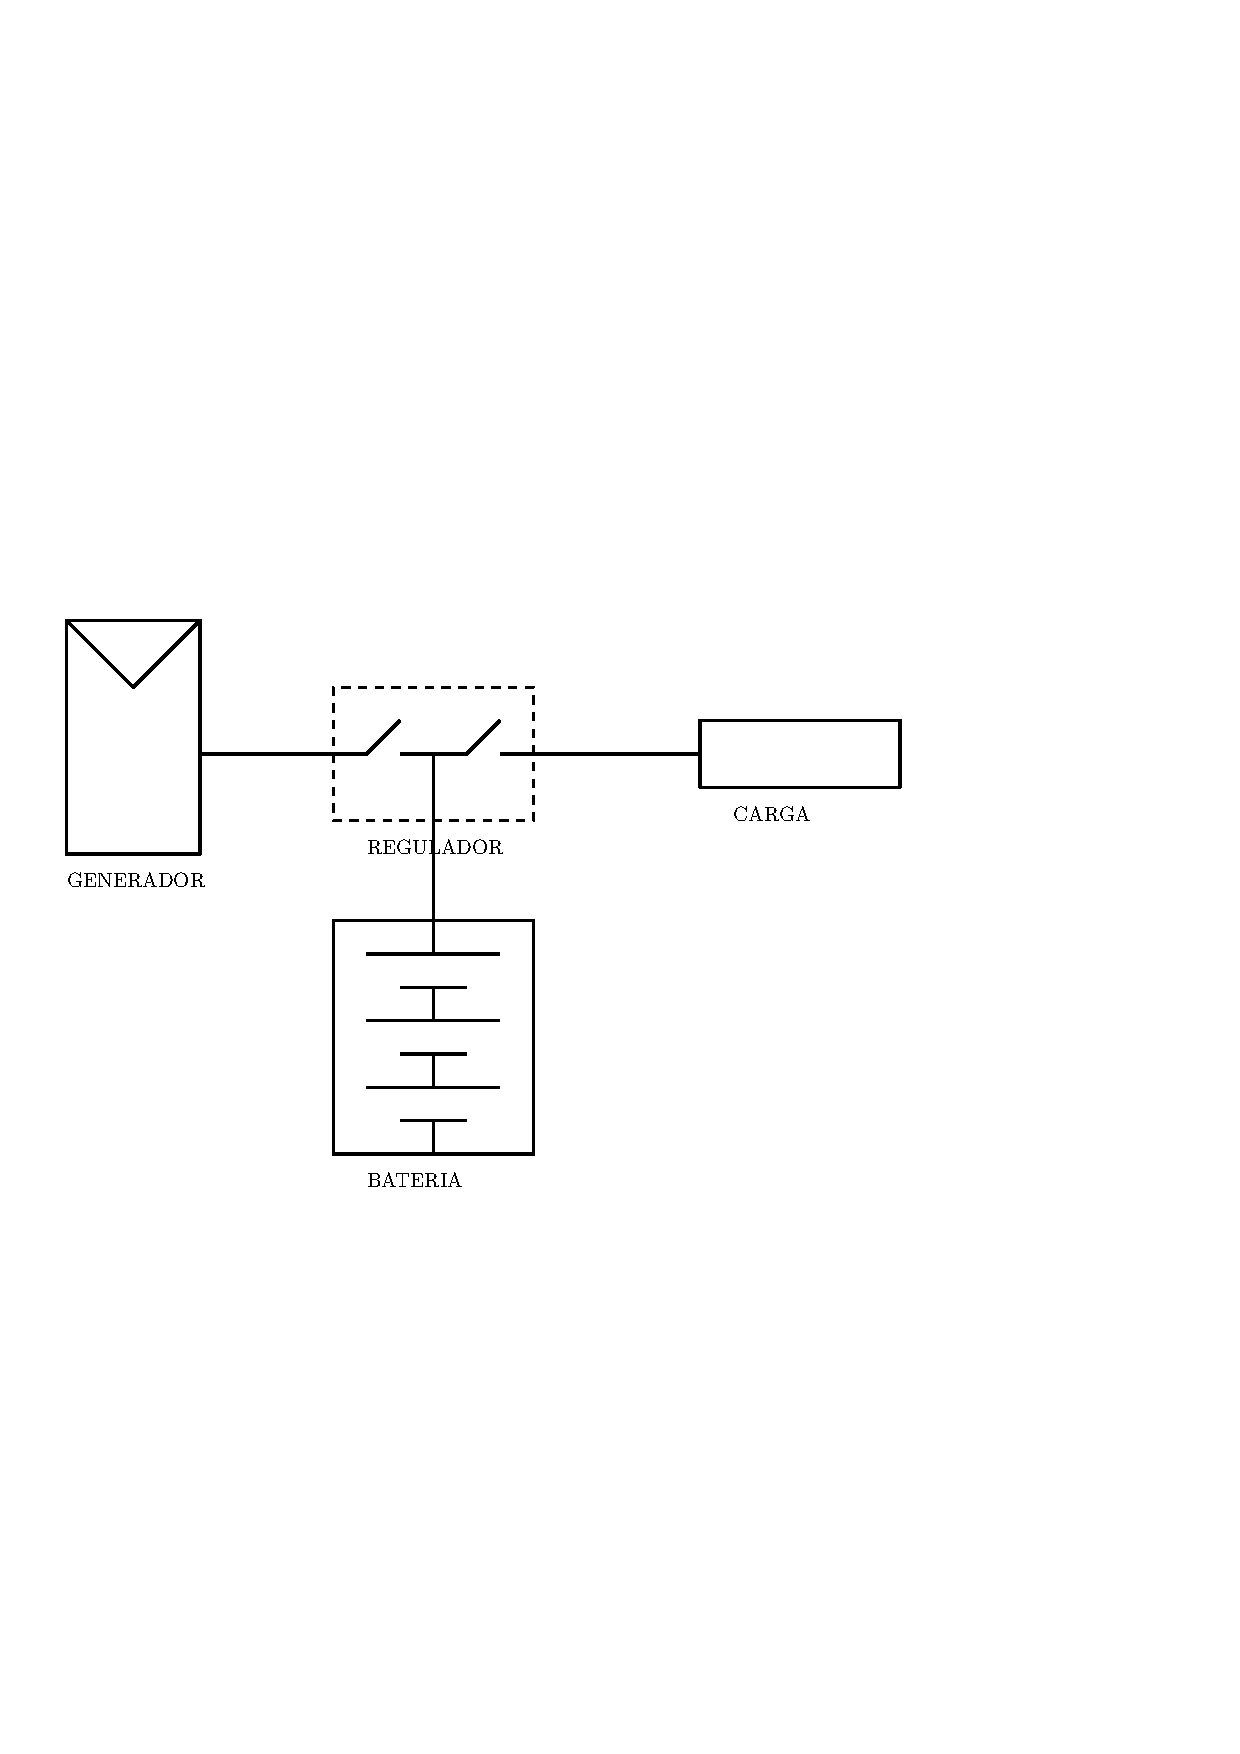
\includegraphics[scale=0.6]{../Figuras/DiagramaUnifilarER_DC}
\par\end{center}


\end{frame}

\begin{frame}
\frametitle{Configuración AC}

\begin{center}
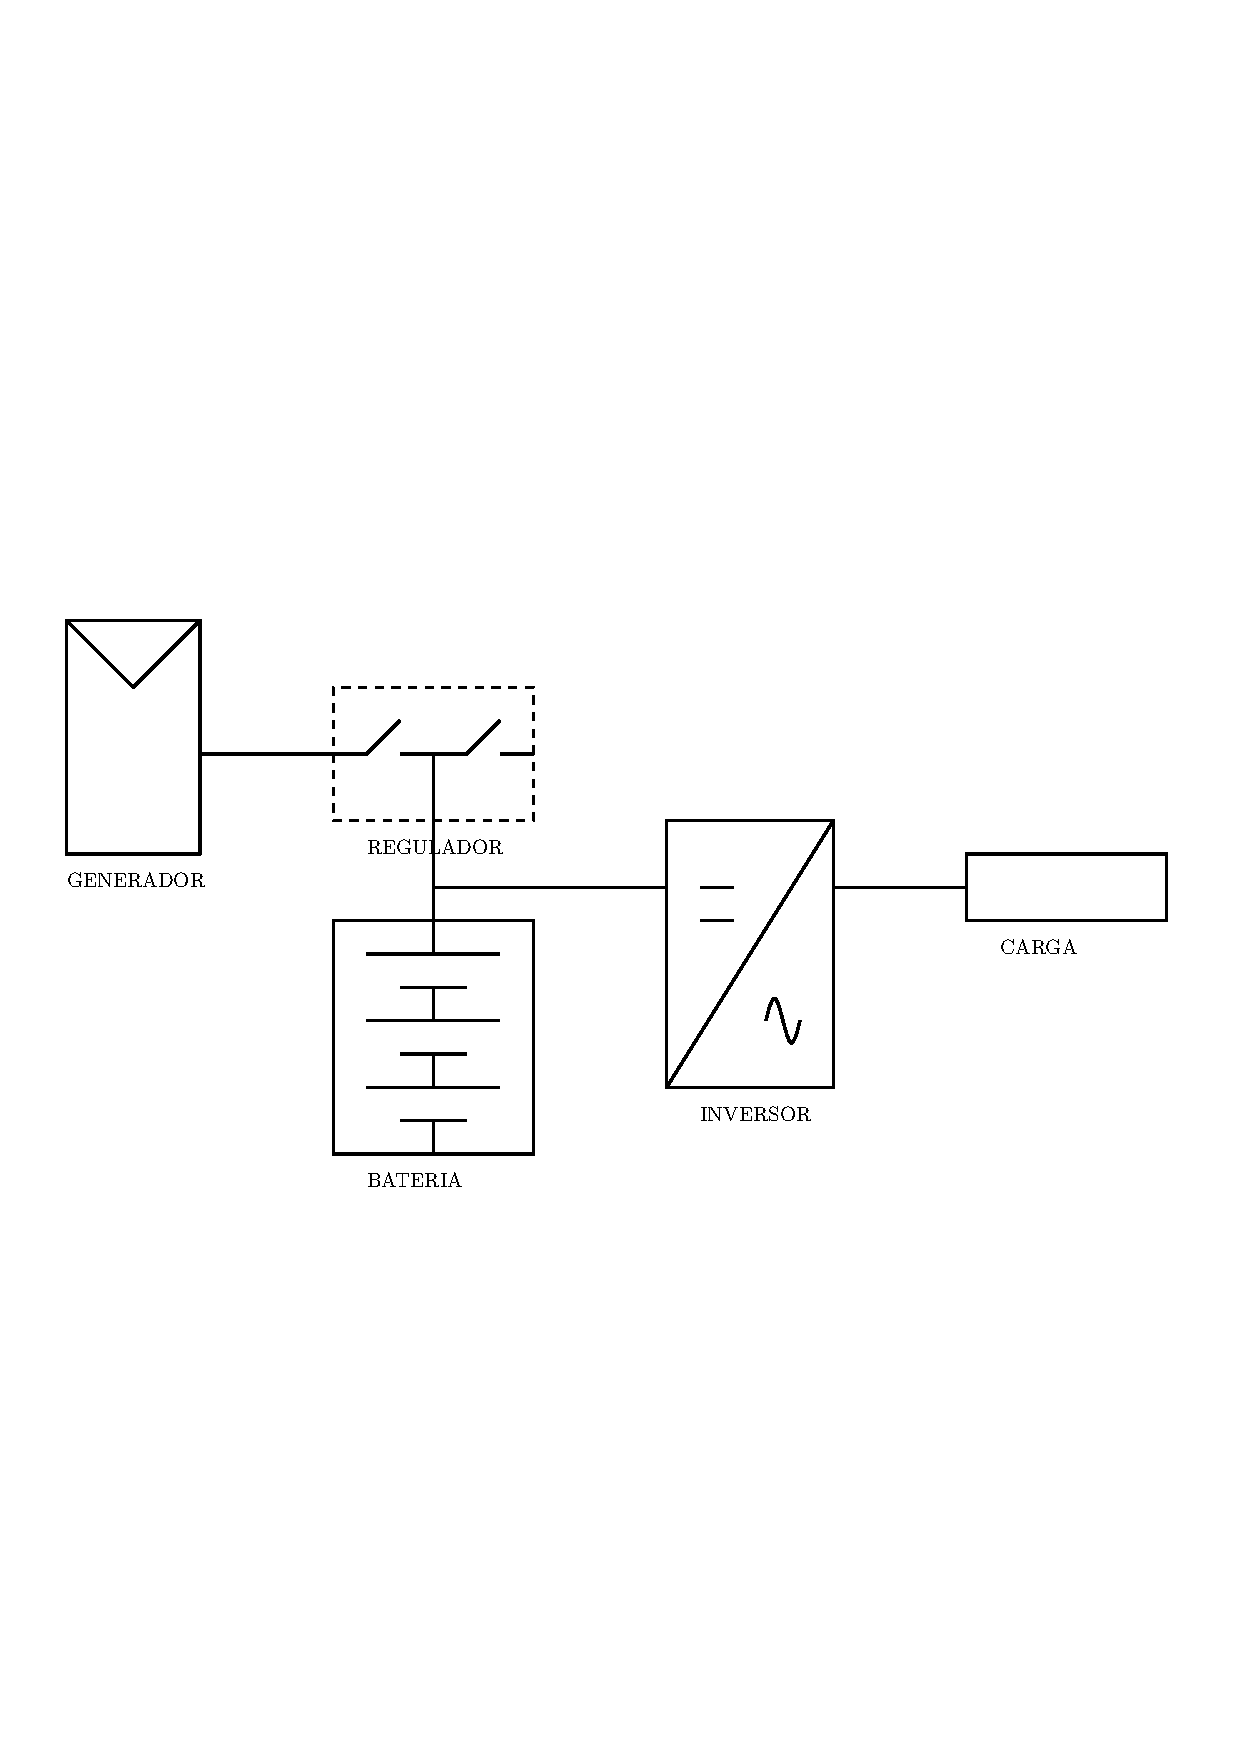
\includegraphics[scale=0.6]{../Figuras/DiagramaUnifilarER_AC}
\par\end{center}


\end{frame}

\begin{frame}
\frametitle{Configuración DC+AC}

\begin{center}
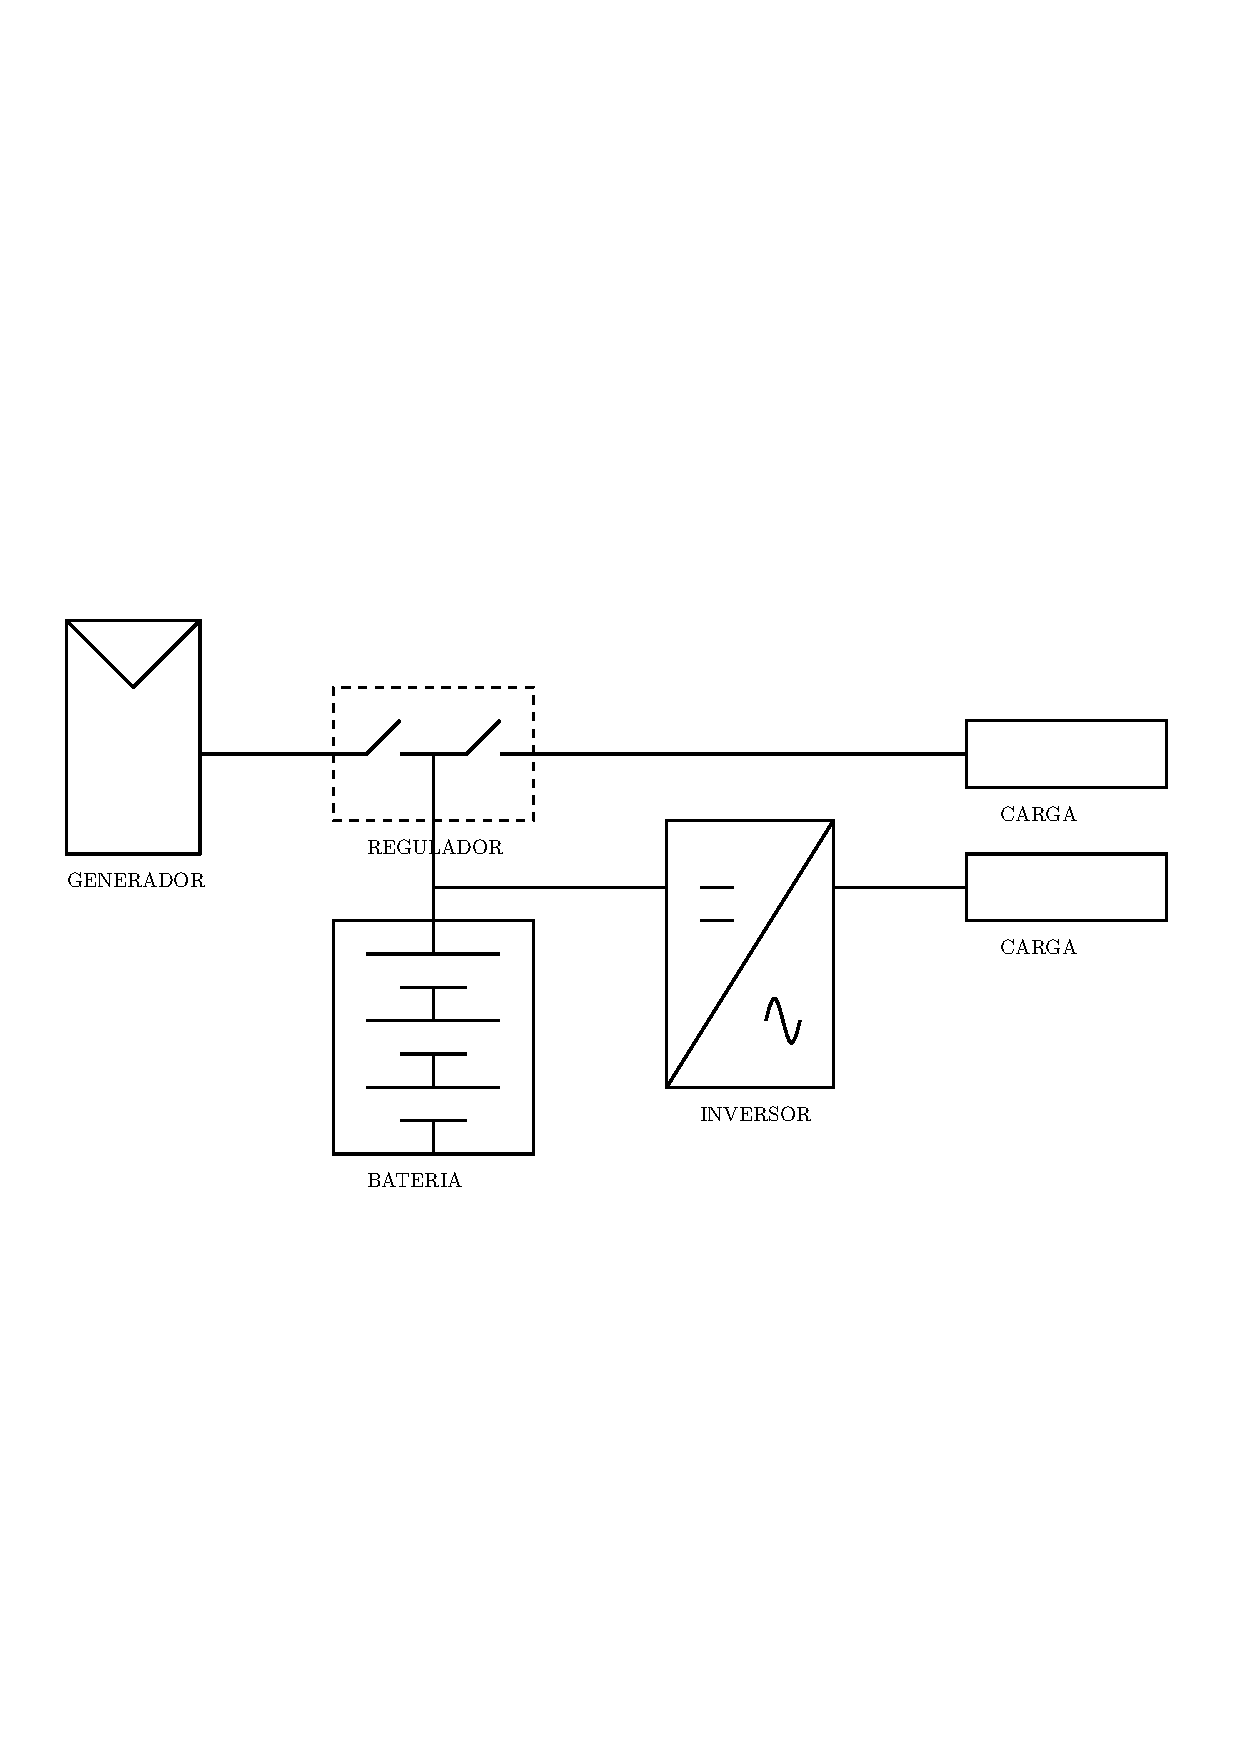
\includegraphics[scale=0.6]{../Figuras/DiagramaUnifilarER_AC_DC}
\par\end{center}


\end{frame}

\begin{frame}
\frametitle{Sistema Híbrido}

\begin{center}
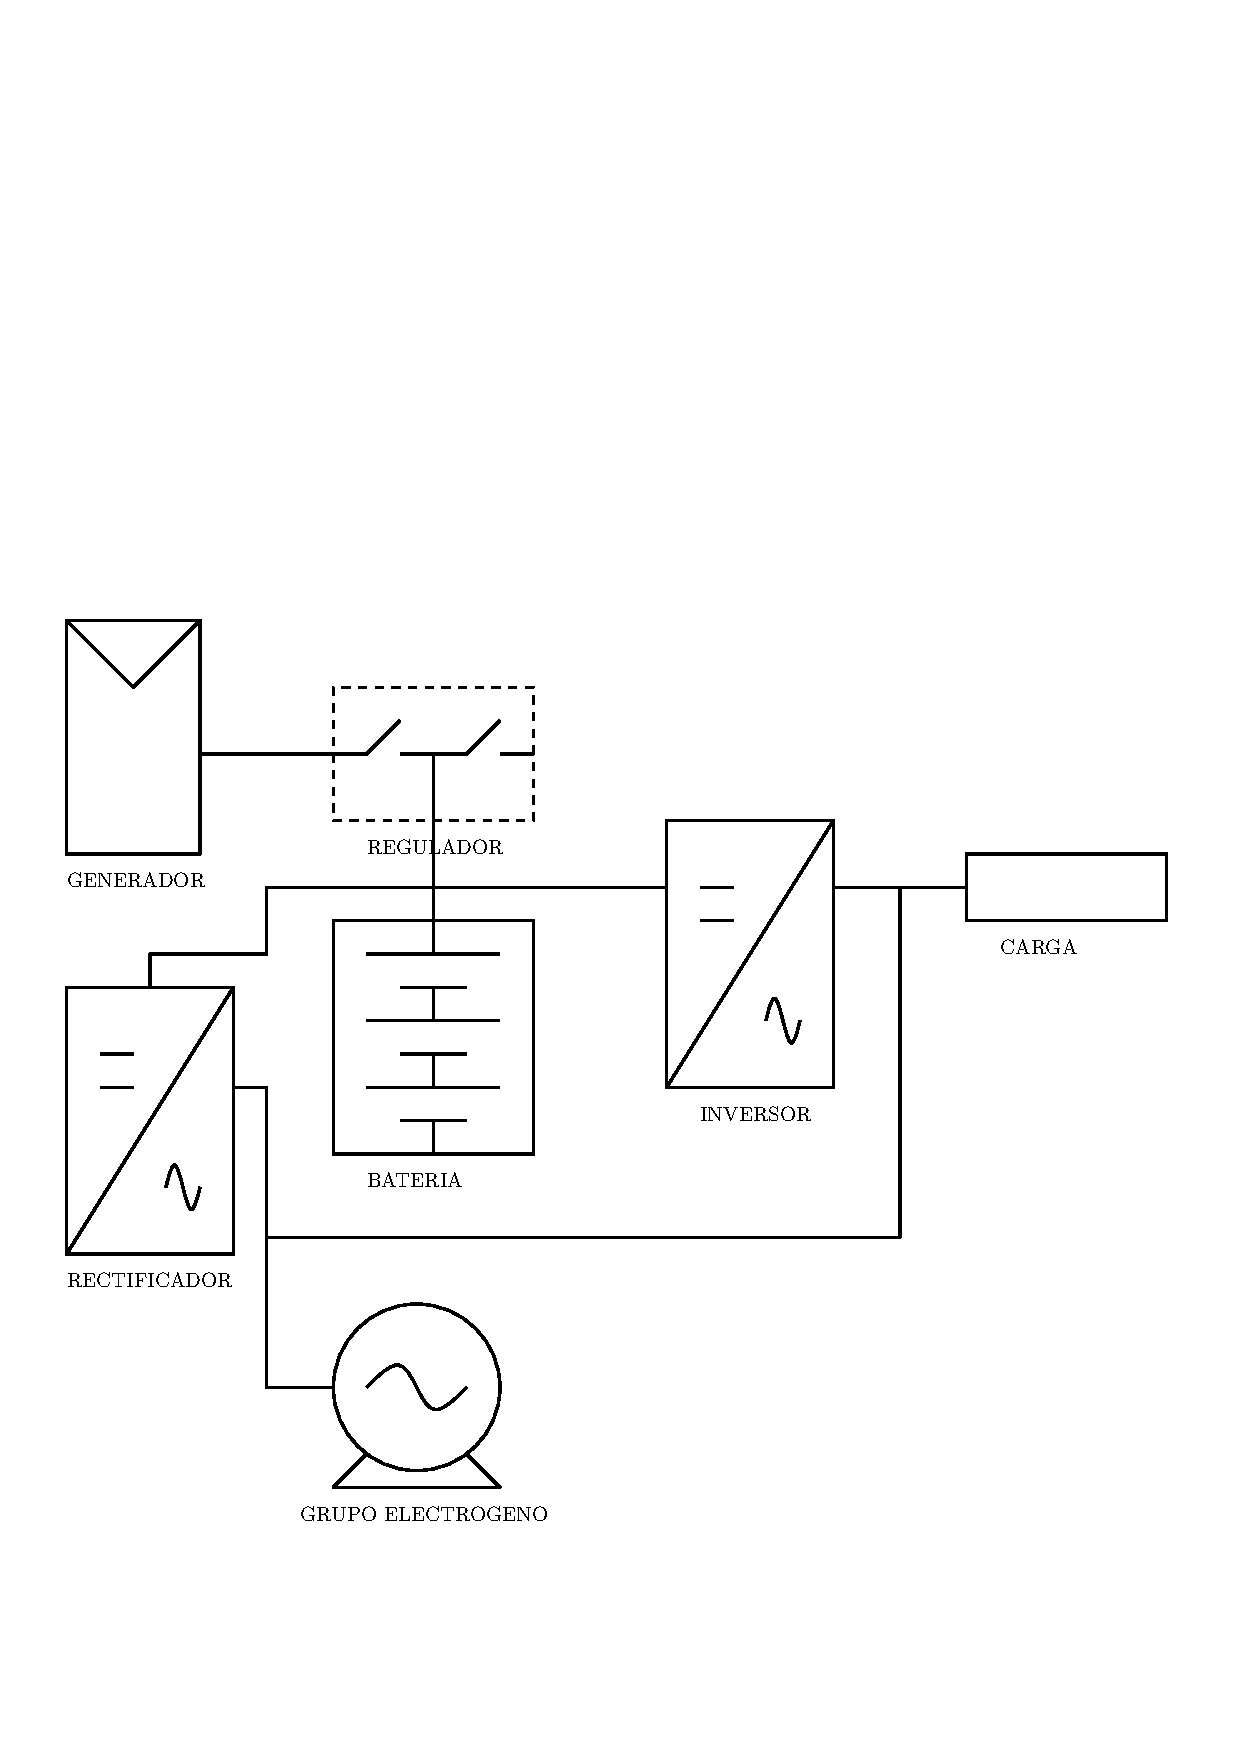
\includegraphics[scale=0.45]{../Figuras/DiagramaUnifilarER_Hibrido}
\par\end{center}


\end{frame}

\section{Acumulador Electroquímico}


\subsection{Definiciones}


\begin{frame}
\frametitle{Acumulador electroquímico}

Un acumulador electroquímico es una bateria secundaria o recargable,
capaz de almacenar energía eléctrica mediante una transformación en
energía electroquímica. Sus principales funciones son:
\begin{itemize}
\item \textbf{Autonomía}: satisface los requerimientos de consumo en cualquier
momento, independientemente de la generación.
\item \textbf{Suministro de picos de intensidad}: cuando es necesario, puede
suministrar valores de intensidad superiores a los que proporciona
el generador FV.
\item \textbf{Estabilización del voltaje}: evita fluctuaciones dañinas para
los equipos de consumo.
\end{itemize}

\end{frame}

\begin{frame}
\frametitle{Definiciones}
\begin{description}
\item [{Capacidad~nominal~($C_{nom}$)}] es la carga eléctrica que puede
ser extraída de una batería hasta llegar a la descarga total.
\item [{Régimen~de~carga/descarga}] es la corriente aplicada a una batería
para restablecer/extraer la capacidad nominal. Normalmente se presenta
como un ratio entre la capacidad nominal y la corriente. 
\item [{Estado~de~carga~(SoC)}] de una batería es la capacidad de una
batería parcialmente cargada, dividida por su capacidad nominal. Por
tanto siempre será $0<SoC<1$.
\end{description}

\end{frame}

\begin{frame}
\frametitle{Definiciones}
\begin{description}
\item [{Profundidad~de~descarga~(PD)}] es el complemento del estado
de carga.
\item [{Tensión~de~corte:}] es la tensión a la que finaliza la descarga
de la batería. Depende del régimen de descarga y del tipo de batería.
Determina la profundidad de descarga máxima, $PD_{max}$, y por tanto,
la capacidad útil, $C_{U}$, siendo \[
C_{U}=PD_{max}\cdot C_{nom}\]

\end{description}

\end{frame}

\begin{frame}
\frametitle{Definiciones}
\begin{description}
\item [{Eficiencia~farádica}] es el ratio entre la carga extraída durante
la descarga y la carga requerida para restablecer el estado inicial.
\item [{Eficiencia~energética}] es el ratio entre la energía extraída
durante la descarga y la energía requerida para restablecer el estado
inicial.
\end{description}

\end{frame}

\subsection{Principios de funcionamiento}


\begin{frame}
\frametitle{Principios de funcionamiento}

Una batería de ácido-plomo se compone de:
\begin{itemize}
\item Un \textbf{ánodo o electrodo positivo} con PbO$_{\text{2}}$
\item Un \textbf{cátodo o electrodo negativo} con Pb.
\item \textbf{Electrolito} a base de $H_{2}SO_{4}$ diluido en agua.
\end{itemize}

\end{frame}

\begin{frame}
\frametitle{Principio de funcionamiento}

\textbf{Ánodo (+):}\[
\mathrm{PbO_{2}+SO_{4}^{2-}+H^{+}+2e^{-}\rightleftarrows PbSO_{4}+2H_{2}O}\]


\textbf{Cátodo (-):}\[
\mathrm{Pb+SO_{4}^{2-}\rightleftarrows PbSO_{4}+2e^{-}}\]


\textbf{Global:}\[
\mathrm{Pb+PbO_{2}+2H_{2}SO_{4}\rightleftarrows2PbSO_{4}+2H_{2}O}\]



\end{frame}

\begin{frame}
\frametitle{Modelo de funcionamiento}
\begin{columns}[c]%{}


\column{5cm}

\[
V_{B}=V_{BI}+I_{C}R_{BI}\]


\[
V_{B}=V_{BI}-I_{D}R_{BI}\]


\[
V_{BI}=\rho_{e}+0.84\]



\column{5cm}

\begin{center}
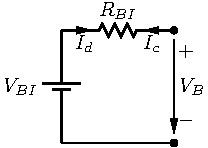
\includegraphics{../Figuras/Bateria}
\par\end{center}

\end{columns}%{}
\begin{block}
{}

Para baterías cargadas, $\rho_{e}$ varia entre $\SI{1.2}{\gram\per\cm\cubed}$
y $\SI{1.28}{\gram\per\cm\cubed}$. Por tanto, la tensión en circuito
abierto de un vaso, $V_{BI}$, está comprendida entre $\SI{2.04}{\volt}$
a $\SI{2.12}{\volt}$.

\end{block}

\end{frame}

\begin{frame}[plain]
\frametitle{Evolución de la tensión en un proceso de carga}

\begin{center}
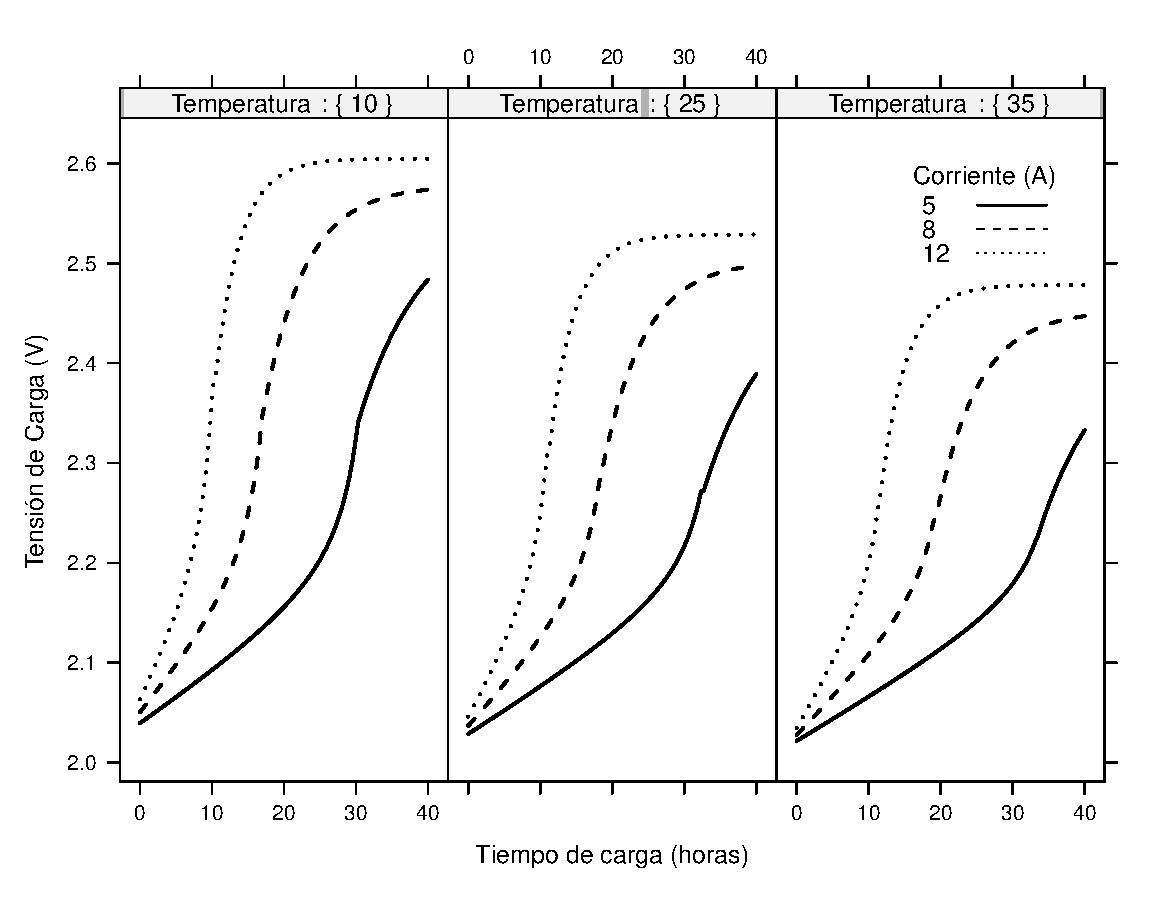
\includegraphics[scale=0.5]{../Figuras/Bateria_CorrYTemp}
\par\end{center}


\end{frame}

\begin{frame}[plain]
\frametitle{Evolución de la tensión durante un proceso de descarga}

\begin{center}
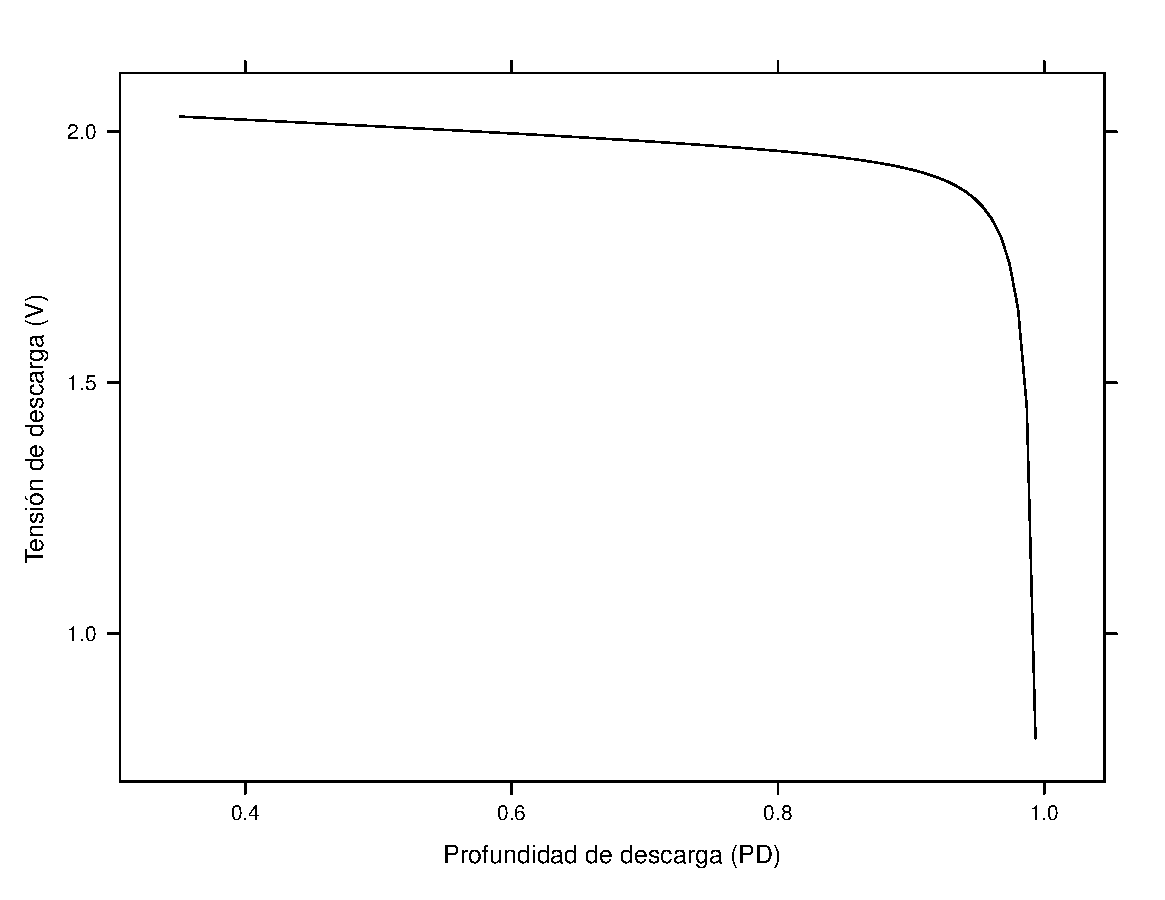
\includegraphics[scale=0.5]{../Figuras/Bateria_SOCyDescarga}
\par\end{center}


\end{frame}

\begin{frame}
\frametitle{Efecto de la temperatura}
\begin{itemize}
\item \textbf{Temperatura baja}:

\begin{itemize}
\item El electrolito se hace más viscoso y decrece la movilidad de los iones
(aumenta la resistencia eléctrica)
\item Baja la capacidad para un regimen de descarga determinado a razón
de 1\%/ºC
\item Si el electrolito se congela, no hay movimiento iónico, y por tanto
la capacidad es nula. Para evitarlo, hay que recurrir a densidades
altas de electrolito en lugares muy frios.
\end{itemize}
\end{itemize}

\end{frame}

\begin{frame}
\frametitle{Efecto de la temperatura}
\begin{itemize}
\item \textbf{Temperatura alta}:

\begin{itemize}
\item Acelera las reacciones, favoreciendo la corrosión. Por tanto, decrece
la vida de la batería.
\item En climas cálidos, se debe optar por bajas concentraciones de electrolito
(que se ve compensada por la mayor movilidad iónica debida a la alta
temperatura).
\item Baja el valor de tensión al que empieza la sobrecarga debido a que
la resistencia interna baja con la temperatura. Hay que corregir el
umbral de corte con la temperatura (se puede utilizar la ambiente
como referencia)
\end{itemize}
\end{itemize}

\end{frame}

\begin{frame}[plain]
\frametitle{Capacidad según el regimen de descarga y la temperatura}

\begin{center}
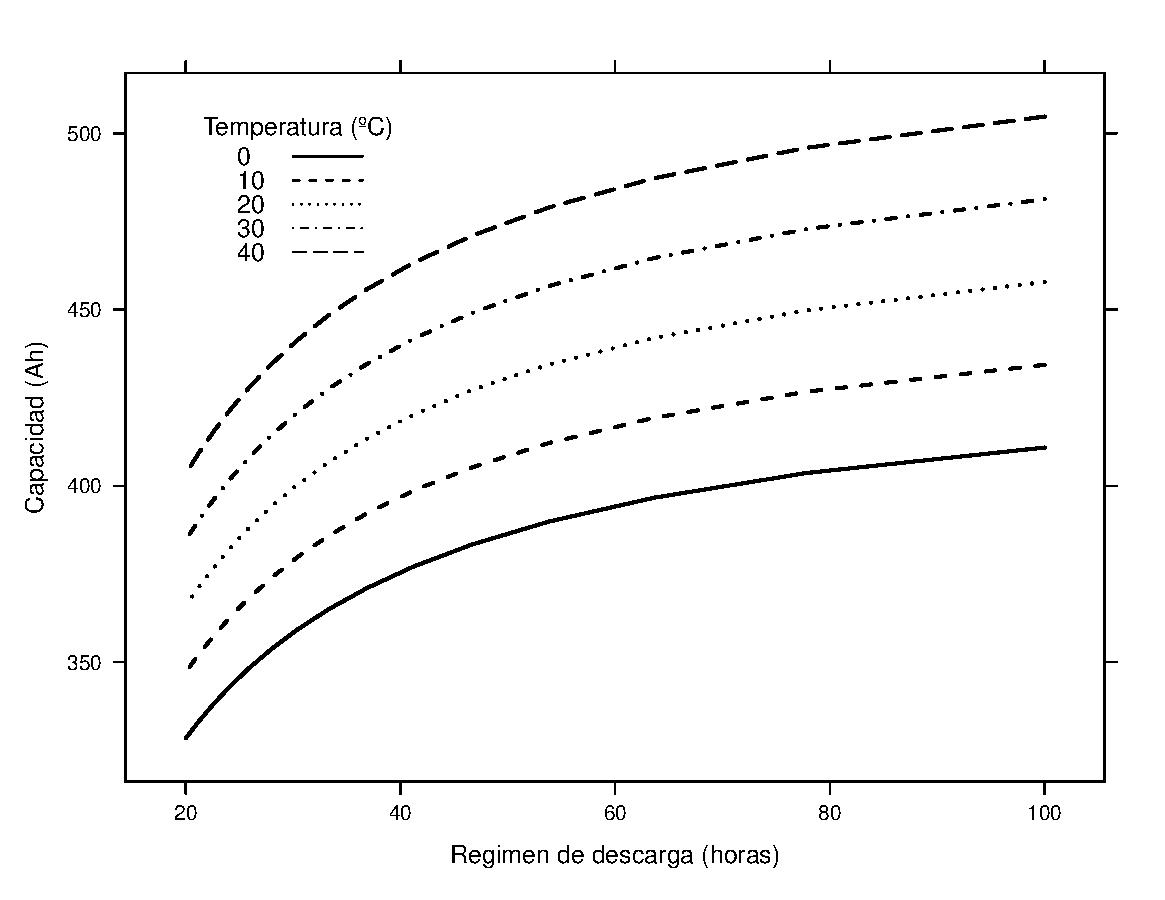
\includegraphics[scale=0.5]{../Figuras/Bateria_Capacidad}
\par\end{center}


\end{frame}

\begin{frame}
\frametitle{Principios de funcionamiento}
\begin{itemize}
\item \textbf{El ciclado es el proceso por el que un acumulador es continuamente
cargado y descargado durante su vida.}
\item \textbf{Durante la descarga}, ambos electrodos transforman la materia
activa en sulfato de plomo en ambos y agua en el ánodo. 

\begin{itemize}
\item Consumo de electrolito (disminuye su densidad) y cambios de volumen
de los materiales activos.
\item Descargas repetidas producen pérdida de material activo y degradación
de las placas. 
\item Si la descarga es muy rápida y la bateria permanece descarga largo
tiempo, el sulfato cristaliza y no es recuperable ({}``sulfatación''). 
\end{itemize}
\end{itemize}

\end{frame}

\begin{frame}
\frametitle{Principios de funcionamiento}
\begin{itemize}
\item \textbf{Durante la carga}, el sulfato de plomo se transforma en oxido
de plomo, plomo y acido. Cuando el proceso de carga está por finalizar
la electrolisis del agua, con liberación de oxigeno e hidrógeno (gaseo)
implica:

\begin{itemize}
\item Pérdida de agua del electrolito (hay que reponerla) 
\item Homogeneización del electrolito por agitación (reduce la estratificación:
mayor concentración de electrolito en zona inferior por gravedad).
\end{itemize}
\end{itemize}

\end{frame}

\begin{frame}
\frametitle{Mecanismos de degradación}
\begin{itemize}
\item \textbf{Corrosión }\textbf{\emph{externa }}\textbf{de los terminales}:
ambientes agresivos. Aumenta la resistencia de contacto, de forma
que la corriente no se distribuye uniformemente entre los vasos que
componen un conjunto acumulador.
\item \textbf{Corrosión }\textbf{\emph{interna}}\textbf{ de las rejillas}:
durante la sobrecarga, el material de las rejillas se degrada, formando
depositos en los vasos. Este fenomeno disminuye la capacidad de forma
irreversible.
\end{itemize}

\end{frame}

\begin{frame}
\frametitle{Mecanismos de degradación}
\begin{itemize}
\item \textbf{Estratificación}: cuando la bateria permanece largos períodos
sin ciclar o en estados parciales de carga, el ácido se concentra
en el fondo, de forma que la densidad del electrolito no es uniforme.
Así, las reacciones no se producen de igual forma en toda la extensión
de las placas. Puede reducirse mediante un gaseo controlado.
\item \textbf{Gaseo excesivo}: produce pérdidas de electrolito y corrosión
en la placa positiva.
\end{itemize}

\end{frame}

\begin{frame}
\frametitle{Mecanismos de degradación}
\begin{itemize}
\item \textbf{Sulfatación}: cuando la batería opera en largos periodos de
carga parcial el sulfato de plomo cristaliza, y deja de participar
en las reacciones químicas, disminuyendo así la capacidad de forma
irreversible. Además, al cristalizar se produce un cambio de volumen
local, provocando tensiones en la rejilla que pueden ocasionar fisuras.
\item \textbf{Depositos de materia activa}: cuando la batería opera en bajos
estados de carga durante largos periodos, la materia activa pierde
adherencia y puede precipitar al fondo del vaso. Además de disminuir
la capacidad, puede ocasionar cortocircuitos que causen la muerte
de la batería.
\end{itemize}

\end{frame}

\begin{frame}
\frametitle{Ciclado}

Factores que influyen sobre la resistencia del acumulador al ciclado
son:
\begin{itemize}
\item \textbf{La profundidad de descarga}: las descargas profundas disminuyen
los ciclos de vida de una batería.
\item \textbf{El régimen de carga}: cuanto mayor es el régimen de carga
y el porcentaje de sobrecarga, menor será la vida alcanzada.
\item \textbf{La temperatura}: las temperaturas altas aceleran la corrosión
en los electrodos disminuyendo los ciclos de vida.
\end{itemize}
El ciclado y los agentes externos contribuyen a degradar el acumulador
hasta que alcanza el fin de su vida útil, momento que puede ser definido
como un valor mínimo en su capacidad útil.


\end{frame}

\subsection{Composición}


\begin{frame}[plain]
\frametitle{Composición}

\begin{center}
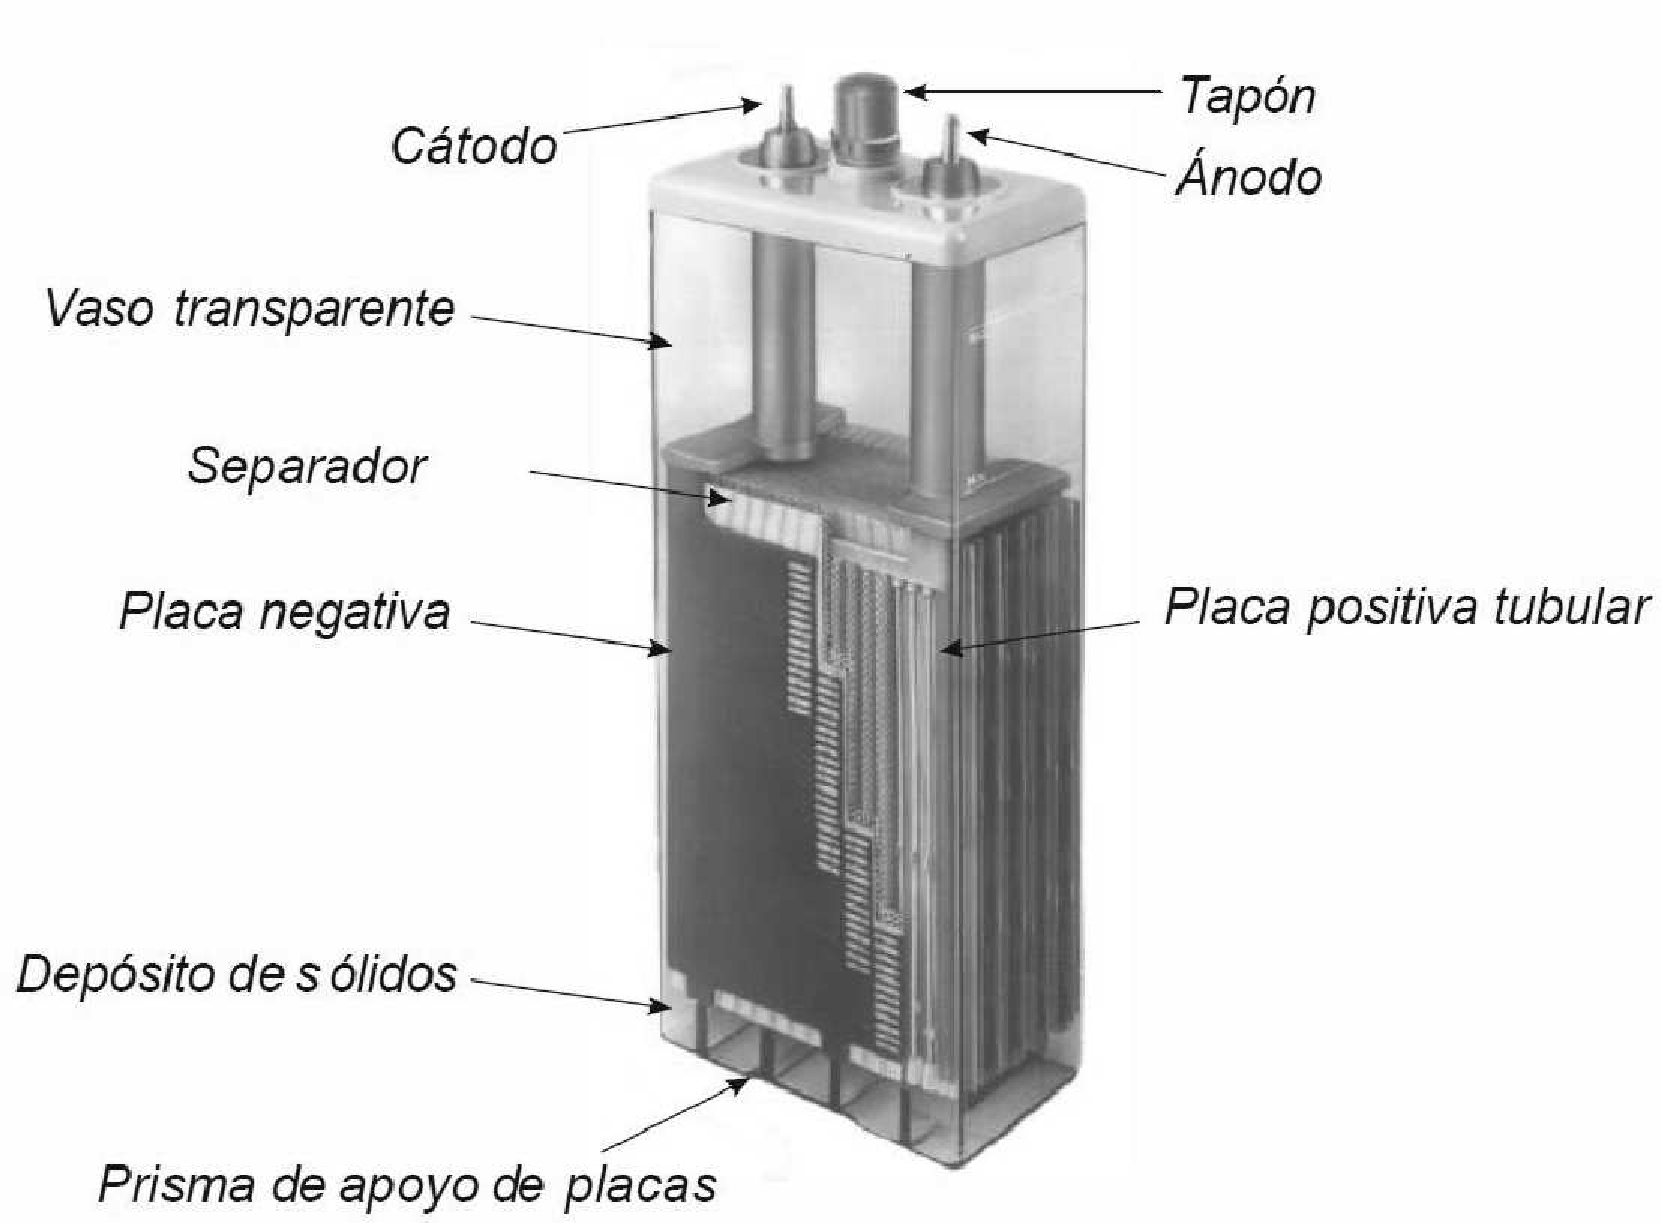
\includegraphics[scale=0.3]{../Figuras/Figuras_Externas/AcumuladorBN}
\par\end{center}


\end{frame}

\begin{frame}
\frametitle{Rejillas}
\begin{itemize}
\item Las rejillas dan \textbf{soporte estructural a los materiales activos}
(oxido de plomo en ánodo, plomo en cátodo) y \textbf{conducen la corriente
eléctrica} hacia el circuito externo. 
\item Están fabricadas en al\textbf{eaciones de Plomo}. 

\begin{itemize}
\item La\textbf{ aleación de plomo-calcio} proporciona alta resistencia
a la corrosión por sobrecarga pero presenta elevada corrosión en bajos
estados de carga. 
\item La \textbf{aleación de plomo-antimonio} presenta buen comportamiento
en ciclado y en descarga profunda. 
\end{itemize}
\item \textbf{La rejilla negativa es plana}, mientras que la \textbf{rejilla
positiva puede ser plana} (operación en flotación) \textbf{o tubular
}(operación en ciclado).
\end{itemize}

\end{frame}

\begin{frame}
\frametitle{Materiales activos y electrolito}
\begin{itemize}
\item Los materiales activos participan en las reacciones químicas. Están
a\textbf{dheridos a las rejillas}. Deben ser \textbf{porosos} para
permitir la penetración del electrolito
\item El \textbf{electrolito} participa en la reacción y \textbf{realiza
el transporte iónico }para cerrar el ciclo de corriente de las reacciones. 
\item La \textbf{elección del electrolito} debe tener en cuenta su \textbf{densidad,
conductividad, punto de congelación, poder de corrosión e impurezas}. 
\end{itemize}

\end{frame}

\begin{frame}
\frametitle{Electrolito}
\begin{itemize}
\item \textbf{Para reducir la resistencia eléctrica del electrolito, su
densidad debe ser alta}, pero \textbf{un electrolito de alta densidad
es muy agresivo} (produce corrosión en la rejilla positiva). 
\item Altos regímenes de descarga requieren mayor densidad para facilitar
el transporte iónico. Los acumuladores estacionarios utilizan densidades
más bajas que los de arranque. 
\item El electrolito \textbf{puede ser líquido} (aireadas) \textbf{o inmovilizado}
(selladas).
\end{itemize}

\end{frame}

\begin{frame}
\frametitle{Separadores}
\begin{itemize}
\item Los separadores \textbf{aislan las placas de diferente polaridad pero
permiten el movimiento iónico a través suyo}. Deben tener resistencia
mecánica, ser permeables y porosas, resistentes a la oxidación, sin
contaminantes y electricamente no conductores.
\end{itemize}

\end{frame}

\subsection{Tipos de acumuladores}


\begin{frame}
\frametitle{Características generales}
\begin{itemize}
\item Un acumulador incorporado a un SFA debe ser \textbf{capaz de funcionar
sometido a ciclados diarios y anuales de carga y descarga}, teniendo
en cuenta que la carga entregada por el generador depende directamente
de la radiación (variable en los períodos intradiario e intraanual). 
\item Debido a las posibles fluctuaciones en la carga aportada, es probable
que se sucedan \textbf{periodos prolongados en carga parcial}. 
\item Es habitual que las \textbf{descargas sean a baja intensidad con periodos
de descarga largos}, típicamente en torno a las 100 horas.
\end{itemize}

\end{frame}

\begin{frame}
\frametitle{Baterías de arranque}
\begin{block}
{}
\begin{itemize}
\item Habitualmente empleadas en automóviles
\item Fácilmente localizables en cualquier mercado local a bajo precio (relativo)
\item Opción frecuentemente empleada en sistemas de electrificación rural
de pequeño tamaño
\item Reemplazo de baterías estropeadas
\item Buen comportamiento en descarga de alta intensidad y tienen buen rendimiento
de descarga a bajas temperaturas. 
\item No son resistentes frente al ciclado
\end{itemize}
\end{block}

\end{frame}

\begin{frame}
\frametitle{Baterías de tracción}
\begin{block}
{}
\begin{itemize}
\item Empleadas, por ejemplo, en carretillas elevadoras. 
\item Resistencia suficiente para soportar un elevado número de ciclos profundos
de carga-descarga. 
\item Requieren aportación de agua y mantenimiento frecuente.
\item Empleo en SFA sólo cuando exista mantenimiento regular.
\end{itemize}
\end{block}

\end{frame}

\begin{frame}
\frametitle{Baterías estacionarias}
\begin{block}
{}
\begin{itemize}
\item Empleadas en sistemas de alimentación ininterrumpida (UPS) o instalaciones
remotas (por ejemplo, radioenlaces). 
\item Funcionan en régimen de flotación. 
\item Gran reserva de electrolito aunque realizan poco uso de agua. 
\item Resistencia a la corrosión y elevada fiabilidad.
\item Opción muy interesante para SFA. Precio más elevado frente a las anteriores
opciones.
\end{itemize}
\end{block}

\end{frame}

\begin{frame}
\frametitle{Baterías {}``fotovoltaicas''}
\begin{block}
{}
\begin{itemize}
\item Baterías SLI modificadas (baratas)
\item Baterías estacionarias modificadas (caras)
\end{itemize}
\end{block}

\end{frame}

\begin{frame}
\frametitle{Elección de batería}

La elección entre uno u otro tipo es un ejercicio que debe tener en
consideración no sólo \textbf{criterios puramente técnicos} sino también
aspectos como el \textbf{coste del sistema}, recursos de \textbf{mantenimiento}
disponibles durante la vida del sistema, \textbf{disponibilidad de
reemplazo} en el mercado local o capacidad de intervención del usuario.
No obstante, \textbf{para aplicaciones fotovoltaicas se recomienda
usar baterías estacionarias aireadas de placa positiva tubular, o
al menos baterías SLI modificadas }(placas más gruesas, mayor cantidad
de electrolito por encima de las placas, más baratas que las estacionarias),
con aleación de Pb-Sb en la rejilla y vaso transparente 


\end{frame}

\section{Regulador de carga}


\begin{frame}
\frametitle{Definición}
\begin{block}
{}

Un regulador de carga es un equipo electronico capaz de \textbf{evitar
la sobrecarga y la descarga excesiva de un acumulador} desconectando
al acumulador del generador o del consumo \textbf{cuando se alcanzan
determinados estados umbral, generalmente determinados por la tensión
en bornes}.

\end{block}

\end{frame}

\begin{frame}
\frametitle{Regulador Serie y paralelo}
\begin{block}
{Regulador Serie}

\begin{center}
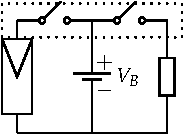
\includegraphics{../Figuras/ReguladorSerie}
\par\end{center}

\end{block}
{}
\begin{block}
{Regulador Paralelo}

\begin{center}
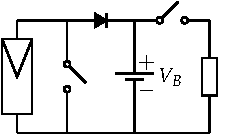
\includegraphics{../Figuras/ReguladorParalelo}
\par\end{center}

\end{block}

\end{frame}

\begin{frame}[plain]
\frametitle{Ciclo de carga}

\begin{center}
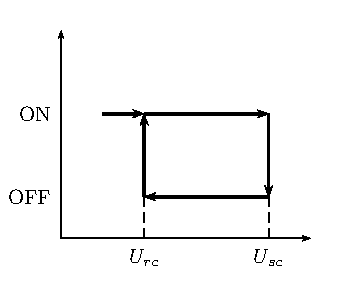
\includegraphics{../Figuras/HisteresisCargaRegulador}
\par\end{center}
\begin{itemize}
\item $U_{sc}$ debe estar en el rango de $\SI{2.3}{\volt}$ a $\SI{2.4}{\volt}$
por vaso a $\SI{25}{\celsius}$. 
\item $U_{rc}$ debe estar en el rango de $\SI{2.15}{\volt}$ a $\SI{2.2}{\volt}$
por vaso a $\SI{25}{\celsius}$. 
\item \textbf{Deben corregirse por temperatura} a razón de $\SI{4}{\milli\volt\per\celsius}$
a $\SI{5}{\milli\volt\per\celsius}$ por vaso.
\end{itemize}

\end{frame}

\begin{frame}[plain]
\frametitle{Ciclo de descarga}

\begin{center}
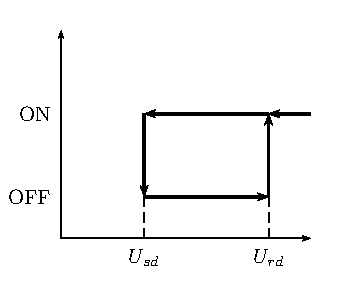
\includegraphics{../Figuras/HisteresisDescargaRegulador}
\par\end{center}

Los umbrales deben adaptarse a cada tipo de batería (mediante ensayos,
o recomendaciones del fabricante)


\end{frame}

\section{Luminarias}


\begin{frame}
\frametitle{Funcionamiento}

Una lámpara fluorescente convencional está formada por un\textbf{
tubo de descarga con gas a baja presión}, un \textbf{recubrimiento
de una mezcla de polvos fluorescentes} y \textbf{dos electrodos} en
los extremos. 

\textbf{Aplicando tensión entre los electrodos}, debido a la ionización
permanente del gas se produce el \textbf{movimiento de las partículas
cargadas} (corriente eléctrica). La \textbf{ionización }permanente
es producida por la radiación exterior, y por tanto, es \textbf{limitada}. 


\end{frame}

\begin{frame}
\frametitle{Funcionamiento}

\textbf{Alcanzado un umbral de tensión, la causa de ionización cambia}:
la tensión aplicada supone un campo eléctrico suficiente como para
comunicar energía a los electrones, que ahora son capaces de ionizar
a los átomos del gas. Este proceso se realimenta y se produce un \textbf{efecto
avalancha}. 


\end{frame}

\begin{frame}
\frametitle{Funcionamiento}

\textbf{A partir de esta etapa, con pequeños incrementos de tensión
la corriente aumenta rápidamente}, hasta alcanzar un límite que ocasiona
un \textbf{arco eléctrico, que debe ser controlado}. Este arco eléctrico
\textbf{afecta al gas}, que emite \textbf{energía electromagnética}
que es \textbf{absorbida por el material fluorescente para producir
radiación en el rango de lo visible}.


\end{frame}

\begin{frame}
\frametitle{Funcionamiento}

Es necesario un \textbf{circuito auxiliar (balasto)} que cumpla dos
funciones principales:
\begin{itemize}
\item \textbf{Proporcionar la tensión de encendido} necesaria para que fluya
corriente por el tubo.
\item \textbf{Regular la corriente} que circula por el tubo una vez que
se ha producido el encendido para evitar su destrucción.
\end{itemize}

\end{frame}

\begin{frame}
\frametitle{Funcionamiento}

\textbf{Al encender el tubo con picos de alta tensión, se produce
desgaste en los electrodos} por el bombardeo iónico. Así, \textbf{el
proceso de encendido es el que más contribuye a la degradación} de
los tubos fluorescentes. Un método alternativo consiste en \textbf{precalentar
los electrodos} (con un circuito basado en un condensador y en una
resistencia) facilitando el paso a la etapa de emisión termoiónica,
y acortando el período de encencedido.

Se recomienda que la lámpara resista un mínimo de 10\,000 ciclos
de encendido y apagado, y en todo caso, \textbf{deberá resistir 5\,000
ciclos.}


\end{frame}

\begin{frame}
\frametitle{Fotometría}
\begin{description}
\item [{Flujo}] radiante es la potencia emitida por la fuente luminosa
(Unidad: Watio)
\item [{Flujo}] luminoso es la potencia emitida capaz de producir sensación
luminosa en el ojo humano (Unidad: Lumen)
\item [{Iluminación}] de una superficie sobre la que incide un flujo luminoso
es el ratio entre flujo y superficie (Unidad: lux, $\si{\lumen\per\watt\squared}$).
\item [{Eficiencia}] de la luminaria (tubo y balasto) es la relación entre
potencia eléctrica consumida por el conjunto y la potencia luminosa
producida (Unidad: $\si{\lumen\per\watt}$). Se recomienda que esta eficiencia
sea superior a 50 $\si{\lumen\per\watt}$, y en todo caso, debe ser superior a 35 $\si{\lumen\per\watt}$.
\end{description}

\end{frame}


\end{document}
